\scanpage{4}
\begin{center}\uline{Imprimeur}\end{center}
\diagram{\begin{tikzcd}[ampersand replacement=\&,column sep=2.4em,row sep=.5em]
\underline{N} \arrow[r,mapsto] \& \mathbb{N}\\
\unsure{\not{1}|\not{l}|\not{\ell}} \arrow[r,mapsto] \& \ell
\end{tikzcd}}
\figure{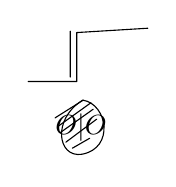
\begin{tikzpicture}[x=.55cm,y=.55cm,line cap=round,line join=round]
\draw (0,0)--(1.12,0)--(1.12,1.13)--(2.76,1.23) (0.97,.10)--(.97,1.16);
\node[inner sep=0pt] at (1.22,-1.07) {$\deleted{\unsure{\mathbb{O}|O}}$};
\draw (1.26,-.43) .. controls (1.83,-.52) and (2.00,-1.54) .. (1.24,-1.68)
 .. controls (.68,-1.77) and (.54,-.87) .. (1.26,-.43);
\draw (.62,-.84)--(1.27,-.43) (.71,-1.02)--(1.45,-.49)
 (.74,-1.18)--(1.50,-.64) (.87,-1.40)--(1.58,-.87)
 (1.02,-1.54)--(1.42,-1.31);
\end{tikzpicture}}
% paper watermark, running down the sheet
\begin{center}\tikz{\node[rotate=-90]{EXTRA STRONG};}\end{center}
\clearpage
% archive sheet number: 3
